% 
% Annual Cognitive Science Conference
% LaTeX Paper -- Proceedings Format
% 

% Original : Jin-Hwa Kim (jhkim@bi.snu.ac.kr)        06/02/2014
% Modified : Jin-Hwa Kim (jhkim@bi.snu.ac.kr)        06/22/2014

%% Change ``a4paper'' in the following line to ``letterpaper'' if you are
%% producing a letter-format document.

\documentclass[10pt,letterpaper]{article}

\usepackage{cogsci}
\usepackage{pslatex}
\usepackage{apacite}

\usepackage{nameref}
\usepackage{graphicx}
\usepackage{subfigure}

\title{Active Long Fixation Correlates with the Formation \\
of Long-Term Memory}
 
\author{{\large \bf Jin-Hwa Kim (jhkim@bi.snu.ac.kr)} \\
  Cognitive Science Program, Seoul National University \\
  Seoul, 151-742, Republic of Korea
  \AND {\large \bf Byoung-Tak Zhang (btzhang@bi.snu.ac.kr)} \\
  School of Computer Science and Engineering, Seoul National University \\
  Seoul, 151-742, Republic of Korea}

\begin{document}

\maketitle

\begin{abstract}
The application of eyewear accelerates the study on the eye movement, for the eye movement is a non-invasive and convenient indicator of the brain activities. We investigate the eye movements of the subjects watching the kids video. We analyze the video sequences by classifying them into two different sequence groups that have the long and short fixation duration, respectively. First, we conduct the long-term memory test of whether fixation duration correlates with long-term memory. Second, we classify its visual constraints into alert and no alert types. As a result of the test, the fixation duration itself is not decisive. However, the long fixations which are actively engaged with alert type movie clips statistically have higher scores, while the short fixations do not. Finally, we propose a simple computational model using the linear regression of two significant features, saliency scrutiny and fixation duration. It may provide an explanatory way to the efficient memory mechanism for the life-long sequences.

\textbf{Keywords:} 
Eye movement; fixation; spatio-temporal; long-term memory, computational modeling.
\end{abstract}



\section{Introduction}

The brain is the most intelligent organ of a living thing. It receives many different forms of sensory information and processes this information appropriately with regard to its survival and reproduce. Especially, the visual information takes a very special position among other kinds of sensory information as it does not need to sense a source directly but is transfered to a remote target far freely than any other types of the sense. Furthermore it gives more chance to survive in the situation of being threaten by the predators using the eyes to detect the foes in the remote place before their approaching. 

But this notable advantage is not freely given one as it requires more delicate and clever way of interpreting the visual information. Because the visual information can easily be affected by the moment-to-moment environmental changes, heuristic but robust compensation strategies are demanded. Hence, how the brain processes the visual information provides the profound way to study the mechanism that the brain precisely and efficiently processes the most dynamic and enormous sensory information.

There are a lot of studies on the computational modeling for the visual information, which include the visual fragment completion, the scene or object classification and recognition \cite{winn2005,lazebnik2006}, and object tracking \cite{YiWu2013}. These research topics often tend to focus on the objective for each task, not on the implementation of the method how the brain deals with. As a result, the computational approach to the modeling for the visual information processing of the brain is gradually changed to the optimization problem, which hinders the understanding of the human-level information processing abilities. 

Particularly, the object tracking seems to describe how we pay attention to an interesting object, however, the eye movement mostly controlled by the oculomotor system, is more complicated how the brain works for the acquisition of the visual information \cite{Henderson2003}. For instance, in the fixation state, the human eyes only recognize the small portion of the whole sight. If you read this paper from an 8-inch distance fixing on one particular letter, you cannot read outside of next two words or about ten letters which are presented in the para-fovea. For the brain is well-known for its parallel processing on the neural circuits, this sequential notion of eye movement for the visual system would be inefficient for information processing.

The studies on the reading eye movement, which are relatively well studied by psychologists and neuroscientists \cite{Rayner1998,Reichle1998}, reveal the fixation duration is related to the presence of the cognitive process \cite{Rayner1997}, for an instance, observing its correlation with linguistic attributes \cite{Inhoff1986,Rayner1986}.

There is a different aspect of studying on the eye movement for video stimuli. How long the fixation sustains is more constrained by the affective content, i.e. emotional response, context of the content, rather than the reading materials do. And the selection of the next fixation and the direction of a saccadic movement tend to be more liberal than the dominance of horizontal searching of reading does. 

Therefore, the study of the eye movement on the video stimuli has been neglected or avoided due to the research complexities and the methodological difficulties \cite{Tatler2011}. However, the recent advancement of the sensory device, like the Google Glass and the mobile devices for the eye tracking, promotes to study on the video stimuli and even more natural experimental environment, and to implement the research model or applications on those mobile devices. 

We investigate the characteristics of eye movements toward the video stimuli. The basic elements of the eye movements are segregated into the fixation duration and the saccade vector, which consists of the saccade direction and the length of the saccadic movement \cite{Findlay1999,Feng2006}. In this study, we focus on the characteristics of the fixation duration as the evidence of the cognitive process. Moreover, as the sequences which potentially induce the emotional arousal are known for helping to recall the seen movie clips \cite{Cahill1996amyg,Cahill1998baso}, we will see if the arousal effect is asserted by the duration of fixation.



\section{Materials and Methods}
\label{sec:material-and-methods}


\subsection{Experiment 1}

For this study, we prepared the video material \textit{Pororo Season 3}, which is a famous kids video in Republic of Korea. In this video, there are artificial 3D-rendered characters who have marked individualities. \textit{Pororo Season 3 DVD 1} contains the 13 consecutive episodes that each has a single storyline.

We recruit 18 participants with normal vision (11 males, 7 females; 23-31 age), who are voluntarily participate in the study. All participants had not experienced a brain damage or a behavioral disorder. The participants are new to the video, \textit{Pororo Season 3}. Experimental procedures were agreed by the Research Ethics of Seoul National University and the participants signed a consent form.

Participants watched the kids video in the room which has the experimental settings. The room is about 3 square meters surrounding by the opaque curtains. On the side of the room, an wide-screen HDTV (1920x1080 resolution, 885 mm x 500 mm, 16:9 ratio) is installed, and 2.1 channel speakers. Participants are guided to sit down on the comfortable sofa in front of 1.7 m from the TV screen.

Concurrently, the eye movements and the user-perspective scenes are recorded by \textit{Tobii Glasses eye tracker}, the corneal reflection based system with a sampling rate of 30 Hz. We used the \textit{I-VT algorithm} as the fixation filter (system default), which classifies fixations with the velocity threshold, 30 degree per second. Usually, the saccadic eye movements are discriminated with low velocities (less than 100 degree/second) and high velocities (higher than 300 degree/second), so the velocity-based classification is simple but reasonable approach \cite{Salvucci2000}.

We classify the event types of the eye movements into three categories; fixation, saccade and unclassified. The unclassified data is discarded and not used in this study.

\begin{figure}
  \centerline{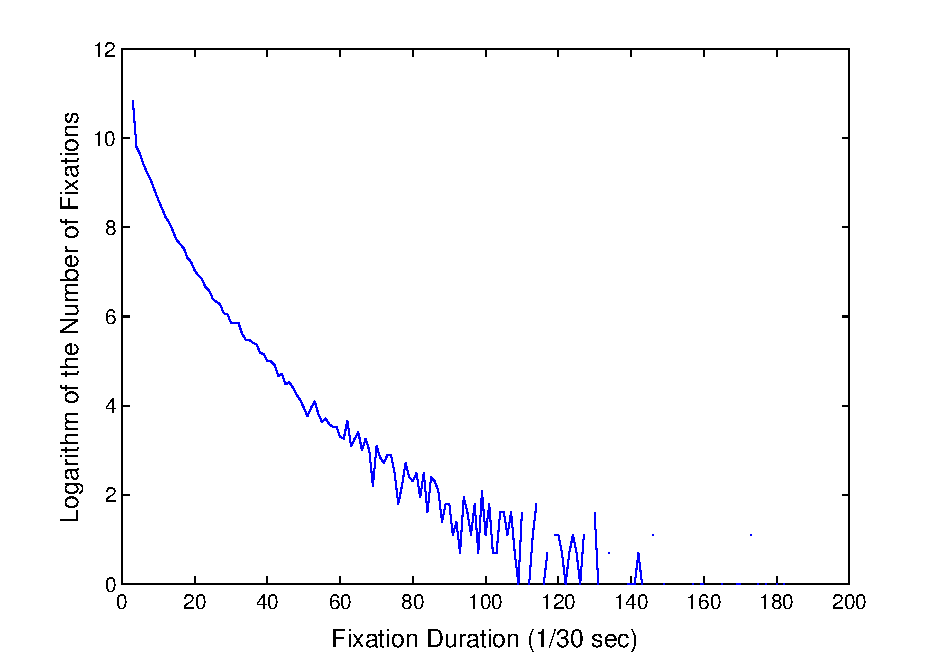
\includegraphics[width=86mm,trim=10mm 3mm 10mm 3mm]{./eps/marginal_fixation_duration.pdf}}
  \caption{The marginal distribution of fixation durations. All of the 158,643 fixation durations of 18 participants is used. The x-axis represents the number of time unit, 1/30 sec., therefore, 30 indicates 1 second. The y-axis represents the logarithm of the number of fixation which have the same time length with regard to the time unit of x-axis.}
  \label{fig:marginal-fixation-duration}
\end{figure}

\begin{figure}
  \centerline{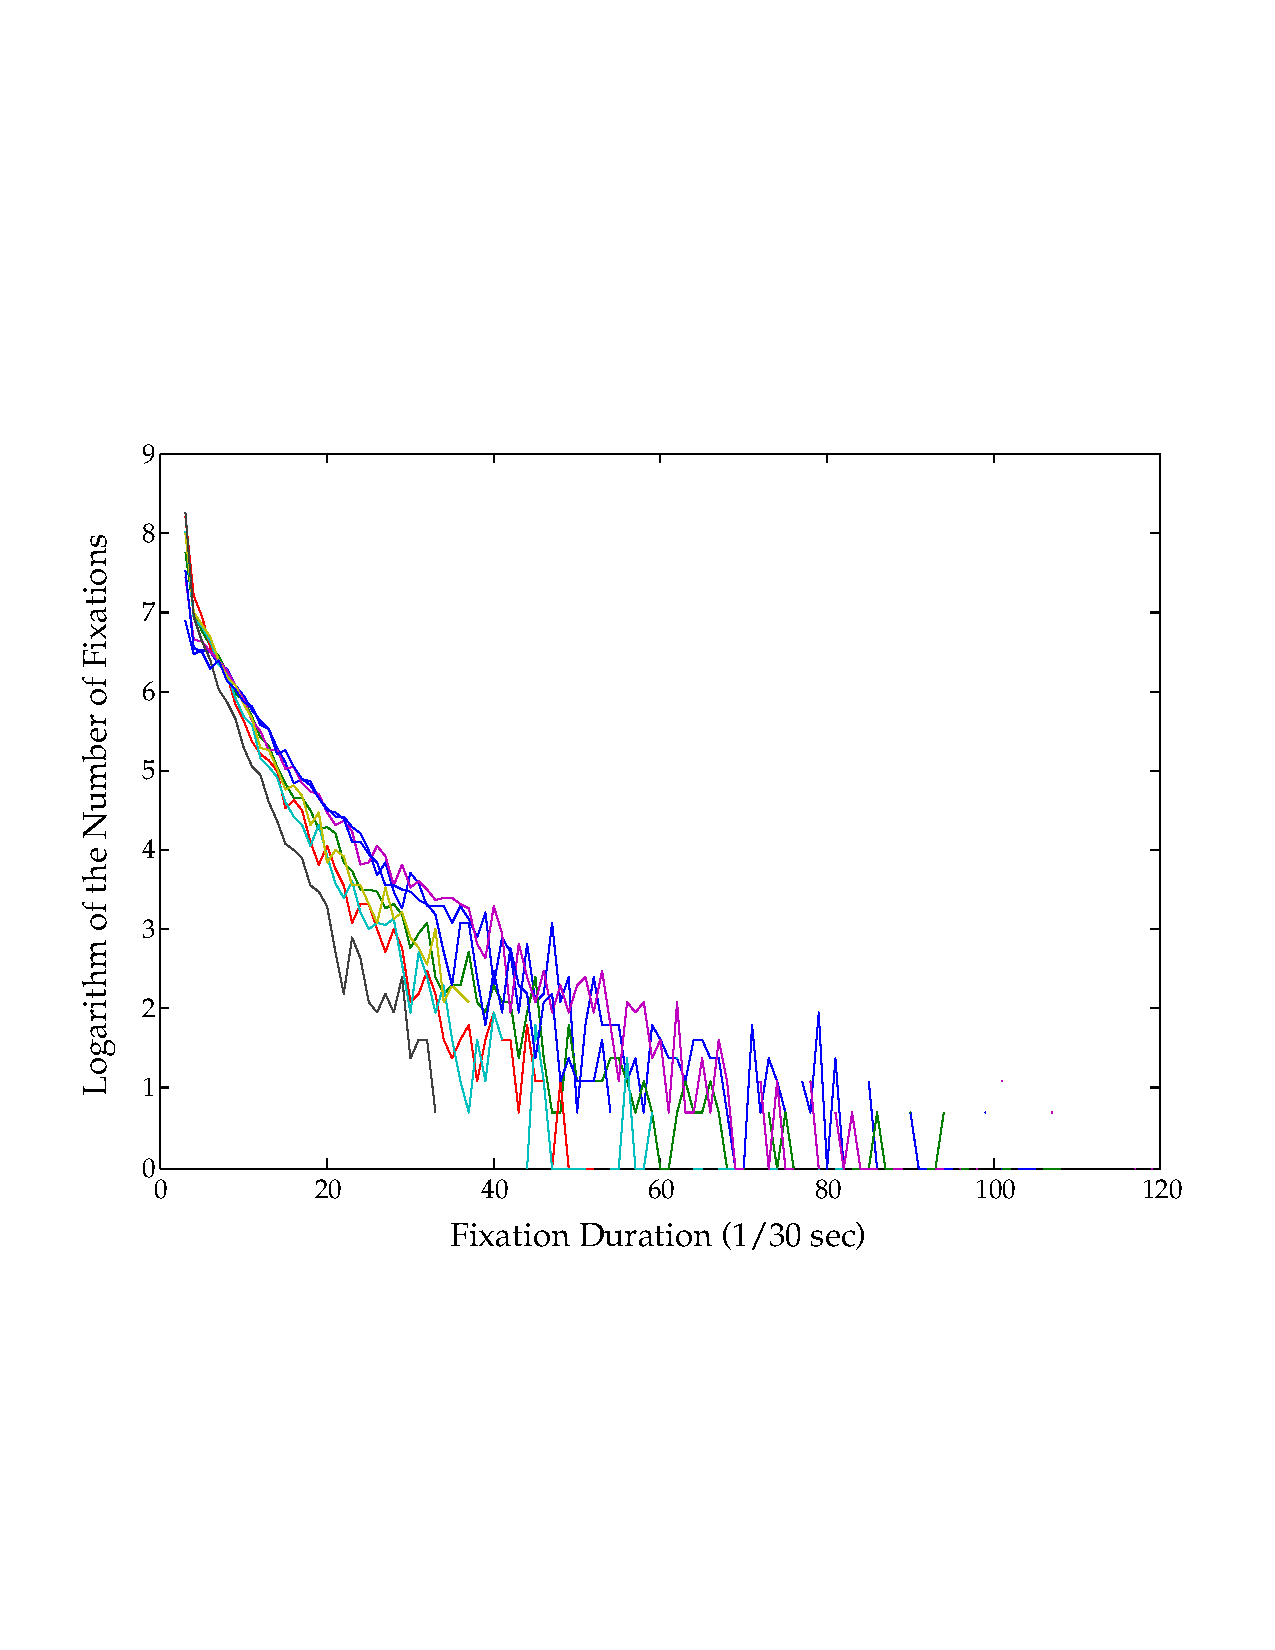
\includegraphics[width=86mm,trim=10mm 3mm 10mm 3mm]{./eps/individual_fixation_duration.pdf}}
  \caption{The distribution of fixation durations for the randomly selected 8 participants. We find the interpersonal differences among all 18 participants, the median of fixation durations varies from 133 ms to 267 ms (mean=183.3, std=41.7).}
  \label{fig:individual-fixation-duration}
\end{figure}


\subsection{Experiment 2}

For 11 participants who have participated in \textit{Experiment 1}, we prepared the controlled memory test for each participant. We conducted this experiment 3-4 months later after \textit{Experiment 1} (the intervals are not consistent due to schedule conflicts). A memory test consists of total 20 video sequences; 8 sequences for long fixations, another 8 sequences for short fixations, and the remaining 4 sequences for the control, which are not seen in the previous experiment. In detail, the lengths of all video sequences are the same as 3 seconds. \textit{The long fixation sequences} are randomly picked from each participant's data containing the fixation longer than 1400 ms in the middle of the sequence. \textit{The short fixation sequences} are randomly picked from each participant's data containing the fixation shorter than 300 ms. The 4 control sequences are randomly picked from the other season of \textit{Pororo} series, \textit{Pororo Season 2}.

Each participant identifies 20 sequences randomly sorted. Each participant gives a sequence 1 to 5 score depending on the assurance of whether he or she saw the sequence before or not. 

\begin{table*}[!ht]
\begin{center} 
\caption{Long Fixation Types.} 
\label{tab:long-fixation-types} 
\vskip 0.12in
\begin{tabular}{ll} 
\hline
Long fixation type    &  Description \\
\hline
Alerted         &   An urgent situation happens with an object, 
                      which can be easily targeted as a cause. \\
Successive      &   Successive changes to keep attracting. \\
Stationary      &   The scene is the same while the target object(s)
                      moves a little or even does not move. \\
Unclassified    &   Cinematic techniques, which are tracking, tilt, 
                      zoom-in and out, and others. \\
\hline
\end{tabular} 
\end{center} 
\end{table*}



\section{Fixation Duration}
\label{sec:fixation-duration}

Fixation duration takes a important position in the reading literature for the durations of eye fixations seems to be constrained by the linguistic features of the fixated word \cite{Rayner1986,Inhoff1986}. In the video watching task, we anticipate the characteristics of fixation duration are different from those in the reading task. As we expect, the fixation duration changes more drastically, up to 10 seconds during watching the video. These changes are partly caused by the sequential changes of the visual stimuli and the fluctuated responses of the oculomotor system and cognitive processes. The length of fixation duration is not a deterministic property, because more than a single component dynamically contribute to the final motor command and the execution for the oculomotor system, we assumed the fixation duration as the random variable with probabilistic distribution \cite{Rayner1998,Reichle2004,Reichle2006}.


\subsection{Marginal Distribution of Fixation Durations}

Figure~\ref{fig:marginal-fixation-duration} shows the marginal distribution of fixation durations, which includes all of the 158,643 fixation durations of 18 participants. The x-axis represents the duration time, and the y-axis represents the log scale of the number of fixations across the whole data.

The shape of the marginal distribution of fixation durations (Figure~\ref{fig:marginal-fixation-duration}) is roughly illustrated as an exponential function. While the distribution of the \textit{reading} fixation durations has a quiet different shape \cite{Feng2006}, segmented into three parts, slow-rising ones for short fixations, fast-rising period until around 180 ms, and following a long tail for long fixation durations. These facts allow us to think that 180 ms of the fixation duration for reading is the most general case, but obviously not for watching the video.

Fixation durations which are longer than about 2 seconds are getting more unpredictable along with increasing the fixation duration. Though it is due to the logarithm increasing the sampling variance, occasionally the content of the video stimuli determines how long the eye gaze is fixated. In other words, the fixation more tends to maintain the gaze position when the visual constraint imposes. The visual constraints have various forms, we will discuss it in subsection~\nameref{subsec:Long-Fixation-Durations}.


\subsection{Individual Distributions of Fixation Durations}

Interpersonal differences are also examined. The individual distributions of fixation durations are shown in Figure~\ref{fig:individual-fixation-duration}. For the analysis, it only shows randomly selected 8 participants' data. The medians of fixation durations from all 18 participants varies from 133 ms to 267 ms with the mean is 183.3 and the standard deviation is 41.7.


\begin{figure*}
  \centerline{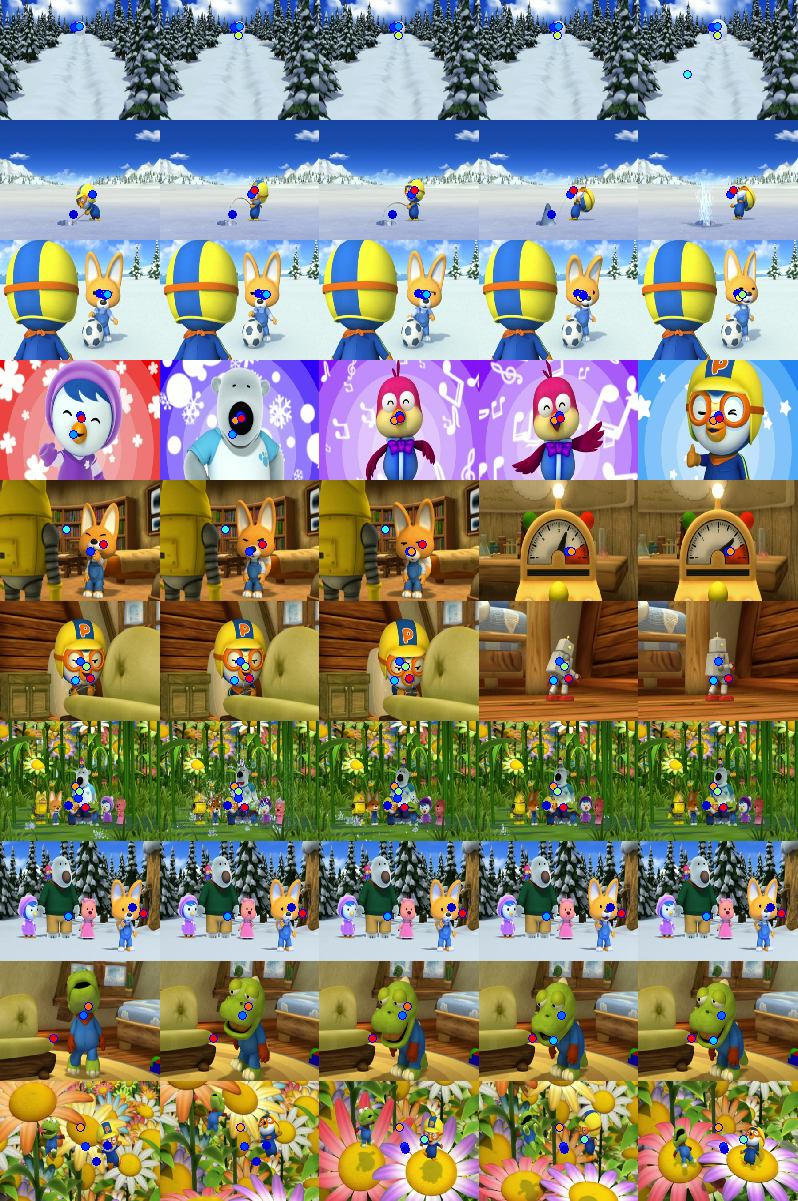
\includegraphics[width=120mm]{./eps/long_fixations_types.png}}
  \caption{The sequences of frames which receive more than 2 seconds of fixation duration from at least 3 participants. Each row means an independent sequence and each column means a single frame. The time interval between frames is 500 ms. The colored dots mean the fixation positions, whose durations are longer than 2 seconds. The same color means what is from the same participant. First 3 sequences show the \textit{Alerted} type, then next 3 sequences show the \textit{Successive} type, then next 3 sequences show the \textit{Stationary} type, and then the last sequence shows the \textit{Unclassified} type of visual constraints for the review. For the description of those sequences, see the text in subsection~\textit{\nameref{subsec:Long-Fixation-Durations}}.}
  \label{fig:long-fixations}
\end{figure*}


\subsection{Long Fixation Durations}
\label{subsec:Long-Fixation-Durations}

In Figure~\ref{fig:long-fixations} the sequences of frames which receive more than 2 seconds of the fixation duration from at least 3 different participants are shown. We set the threshold to reduce the interpersonal variation. We got all 41 sequences across 1 hour 7 minutes 50 seconds length of the material. For the review, we chose 10 typical sequences. Each row means an independent sequence and each column means a single frame. The time interval between the frames is 0.5 seconds. The colored dots mean the fixation positions, whose durations are longer than 2 seconds. The same color means the same participant. Four different types of the sequences are listed as \textit{Alerted} (3), \textit{Successive} (3), \textit{Stationary} (3), and \textit{Unclassified} (1) for the review.

The sequence of the \textit{Alerted} type is classified as the scene implies an unusual and, potentially dangerous or difficult situation, which may introduce a mental arousal. The sequence of the first row demonstrates an urgent moment that a huge snowball is about to roll down back on the hill, which was previously rolled up by the robot, \textit{Rody}. Second shows that \textit{Pororo} has been fishing at the ice hole, but what he caught is \textit{Shark}, a naughty character. Third shows that \textit{Eddy} rolled his eyes to kick his ball avoiding the opponent \textit{Pororo}.

The \textit{Successive} type shows that the fixation duration extends across more than 2 different scenes. Because the location of the target object is not changed or changed within the range of a foveal or central vision, 2-5$^{\circ}$, the fixation holds its position \cite{mcmorris2014acquisition}. The fourth sequence shows the closed-up characters are serially shown up in the center of the screen. The fixations duration of the fifth and sixth sequences extends across different scenes have different visual configurations.

The \textit{Stationary} type most clearly shows the characteristics that the indifferent scene maintains while the target object moves a little bit or even does not move. For there is not a particular event or a change of the scene, the participants tend to fixate their gazes. See the seventh through ninth sequences.

The sequence of the \textit{Unclassified} type takes various forms. The tenth sequence shows that \textit{Pororo} and \textit{Crong} just jumped out of the shoulder of the magician dragon, \textit{Tongtong} who is flying in the sky. Two sunflowers spring \textit{Pororo} and \textit{Crong} into the sky in multiple times. But due to the perspective of the camera, the location of the two characters in the scene is almost fixed. Participants fixated their eye gazes on the center of two characters while the background shifting up and down. In other cases, though not reported in Figure~\ref{fig:long-fixations}, there are cinematic techniques, i.e., tracking, tilt, zoom-in and zoom-out, and other uncertain ones. The number of these cases is relatively so small compared to the other types, hence we classify all of them into the \textit{Unclassified}.



\section{Long-Term Memory Formation}

In the studies of reading eye movements, as noted before, the fixation duration is a good indicator for information processing. The stimulus-response model seems to offer the way of understanding, because a sequence as a stimulus supplies a cause to response, in this case, a long fixation. But we have to be cautious that the long fixation itself is not always induced when the internal state of a subject is positively affected. In addition, the sequences received a long fixation does not decisively guarantee the quality of information processing nor its specificity. When we carefully look into the sequences in Figure~\ref{fig:long-fixations}, the fixations on \textit{Successive} or \textit{Stationary} type sequences can be interpreted as looking passively or even blankly.

This view is also valid for the formation of memory. A stimulus is memorized by the constructive activities, a series of being stimulated, giving attention, and acquisition. But the corresponding responses are not deterministic by the stimulus for the uncertainty of environmental perturbations or the complexity of internal states. Therefore, the formation of memory is the result of the cognitive process of response rather than the response itself. However, the cognitive process is an internal procedure, which only can be measured by the tangible responses indirectly. So, we need to discern the reliable indicator of the cognitive process with a sufficient care.


\subsection{Recall Test}

We define two types of fixation as long and short fixations. The long fixation is the gaze holding its position after fixation filtering longer than 1400 ms. The short fixation is one that shorter than 300 ms. Figure~\ref{fig:memtest-leng} shows the memory test result for the two fixation types. Each participant assessed in a recall test rating 8 long fixated sequences, 8 short fixated sequences and 4 not-seen sequences, which are not seen previously. Contrary to our expectations, the recall scores for the short fixated sequences is not much different from the the recall scores for the long fixated sequences. This result makes sense when we consider that the long fixation is an attentive response, which is actively or passively motivated by a reciprocal process in visual system.

The relationship between the emotional arousal and the formation of long-term memory is known for the studies in neuroscience \cite{Cahill1996amyg,Cahill1998baso}. In this study, we define the emotionally arousal events are urgent, threat, tension, hurt, trouble, surprise or angry situations. On top of this, more detailed analyses are conducted with regard to the type of stimuli.

Figure~\ref{fig:memtest-long} shows The memory test result for the long fixation which is on the \textit{Alert} sequence or the \textit{No Alert} sequence. The \textit{Alert} sequences are classified by the predefined conditions, an unusual and, potentially dangerous or difficult situation, which may introduce an emotional arousal. This classification is rather definite because the content is an animation video for children. Figure~\ref{fig:memtest-alert} shows the result of arousal effect on the recall test, \textit{Alert} sequences significantly get higher recall scores than \textit{No Alert} sequences with the p-value of 0.0077 (p $<$ 0.01). The number of ratings from 11 participants are 19 for the \textit{Alert} and 69 for \textit{No Alert}. The difference between two mean scores for the long and short fixation types is significant. The p-value of two-sample t-test is 0.0104 ($<$ 0.05). The blue horizontal line indicates the mean scores of the long fixated sequences.

Figure~\ref{fig:memtest-short} shows the memory test result for the short fixation types which is on the \textit{Alert} sequences or the \textit{No Alert} sequences. The number of cases from 11 participants are 21 and 67, respectively. The p-value of two-sample t-test is 0.2484 ($>$ 0.05). In the short fixation cases, there is no significance between two content types, \textit{Alert} type and \textit{No Alert} type. The blue horizontal line indicates the mean scores of the short fixated sequences.


\begin{figure}
  \begin{minipage}{.5\textwidth}\centerline{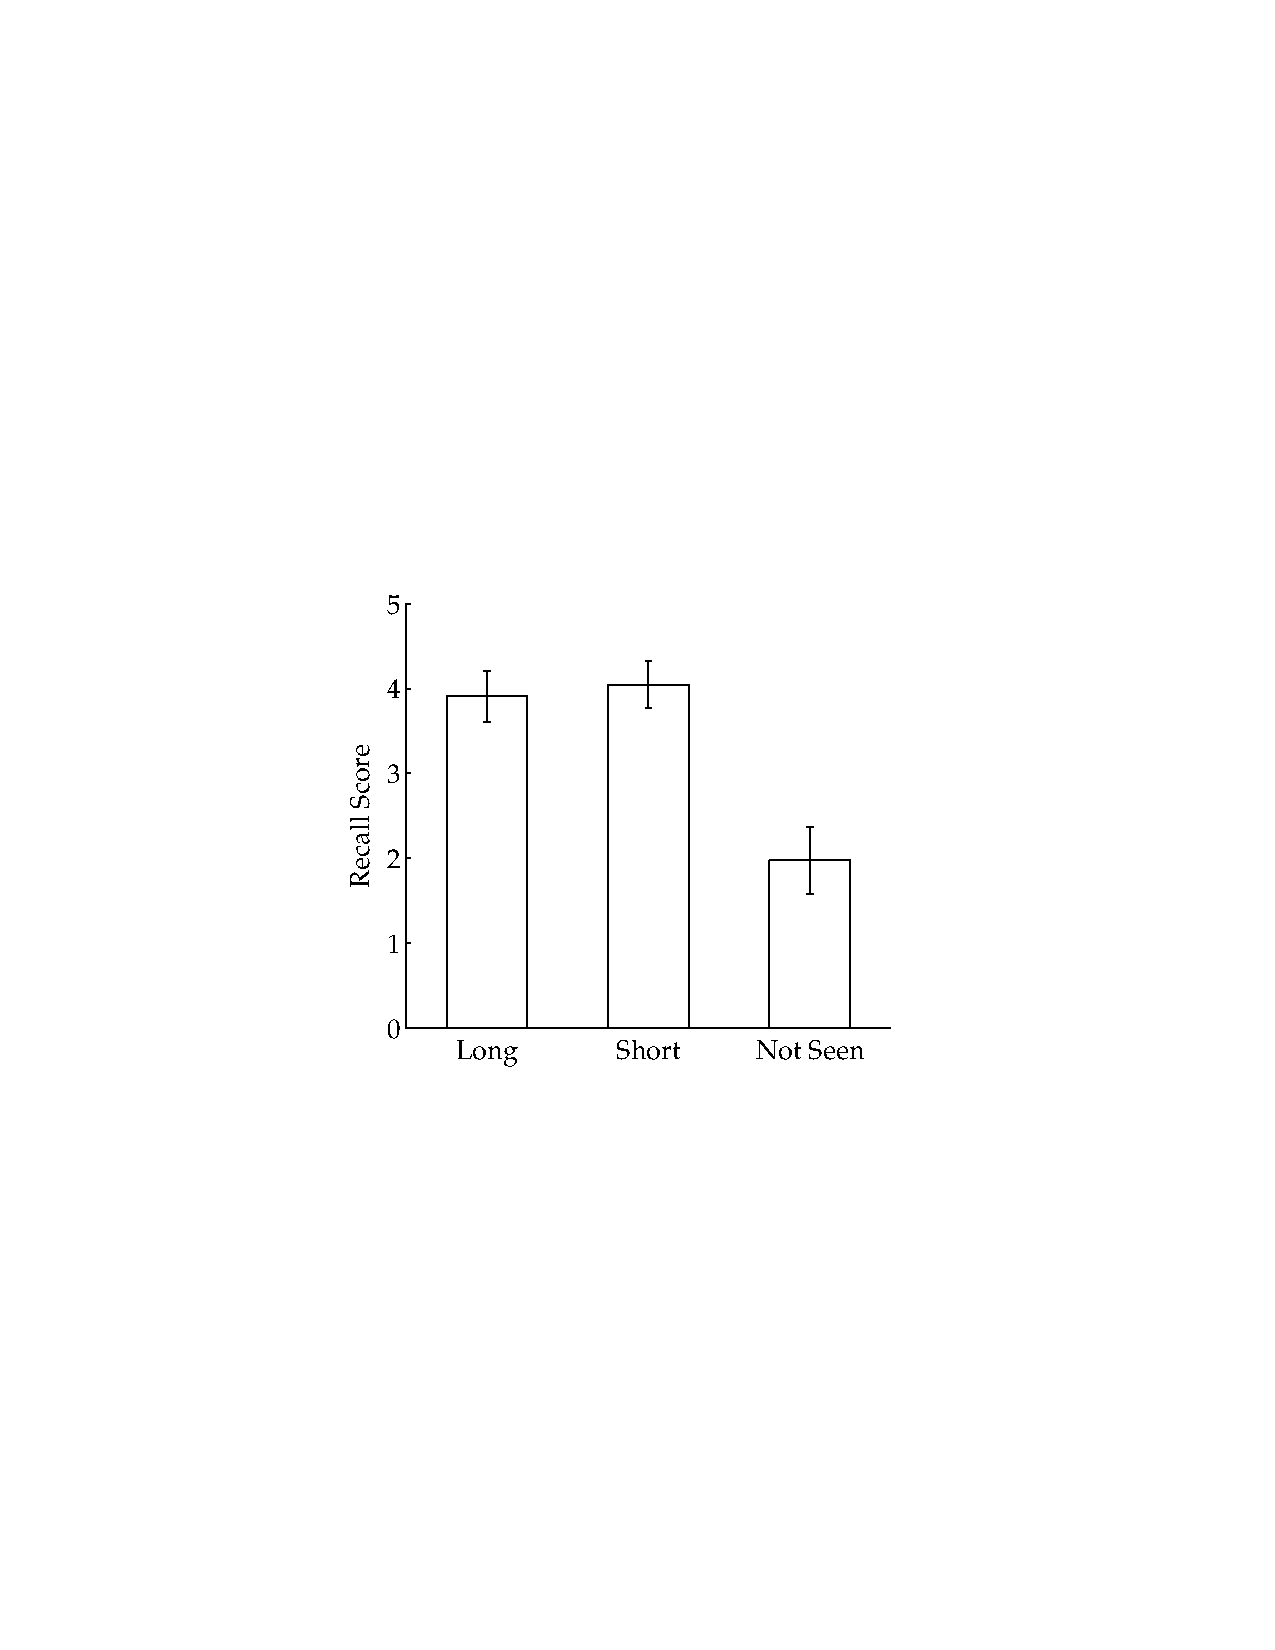
\includegraphics[width=60mm,height=54mm,trim=58mm 110mm 62mm 105mm]{./eps/memtest_leng}}
  \caption{Long-term memory test result for two fixation types, one is that whose duration of fixation is longer than 1400 ms, and the other one is that whose duration of fixation is shorter than 300 ms. Each participant rates 8 long fixated sequences, 8 short fixated sequences and 4 control sequences which are not seen previously. Surprisingly, the mean scores of the short fixated sequences is indifferent to the mean scores of the long fixated sequences (p $=$ 0.5051). Error bars indicate $\pm$ 2 standard errors of means (SEMs). For the detail of test, refer to \textit{\nameref{sec:material-and-methods}}.}
  \label{fig:memtest-leng}
  \end{minipage}
  
  \vskip 0.12in

  \begin{minipage}{.5\textwidth}\centerline{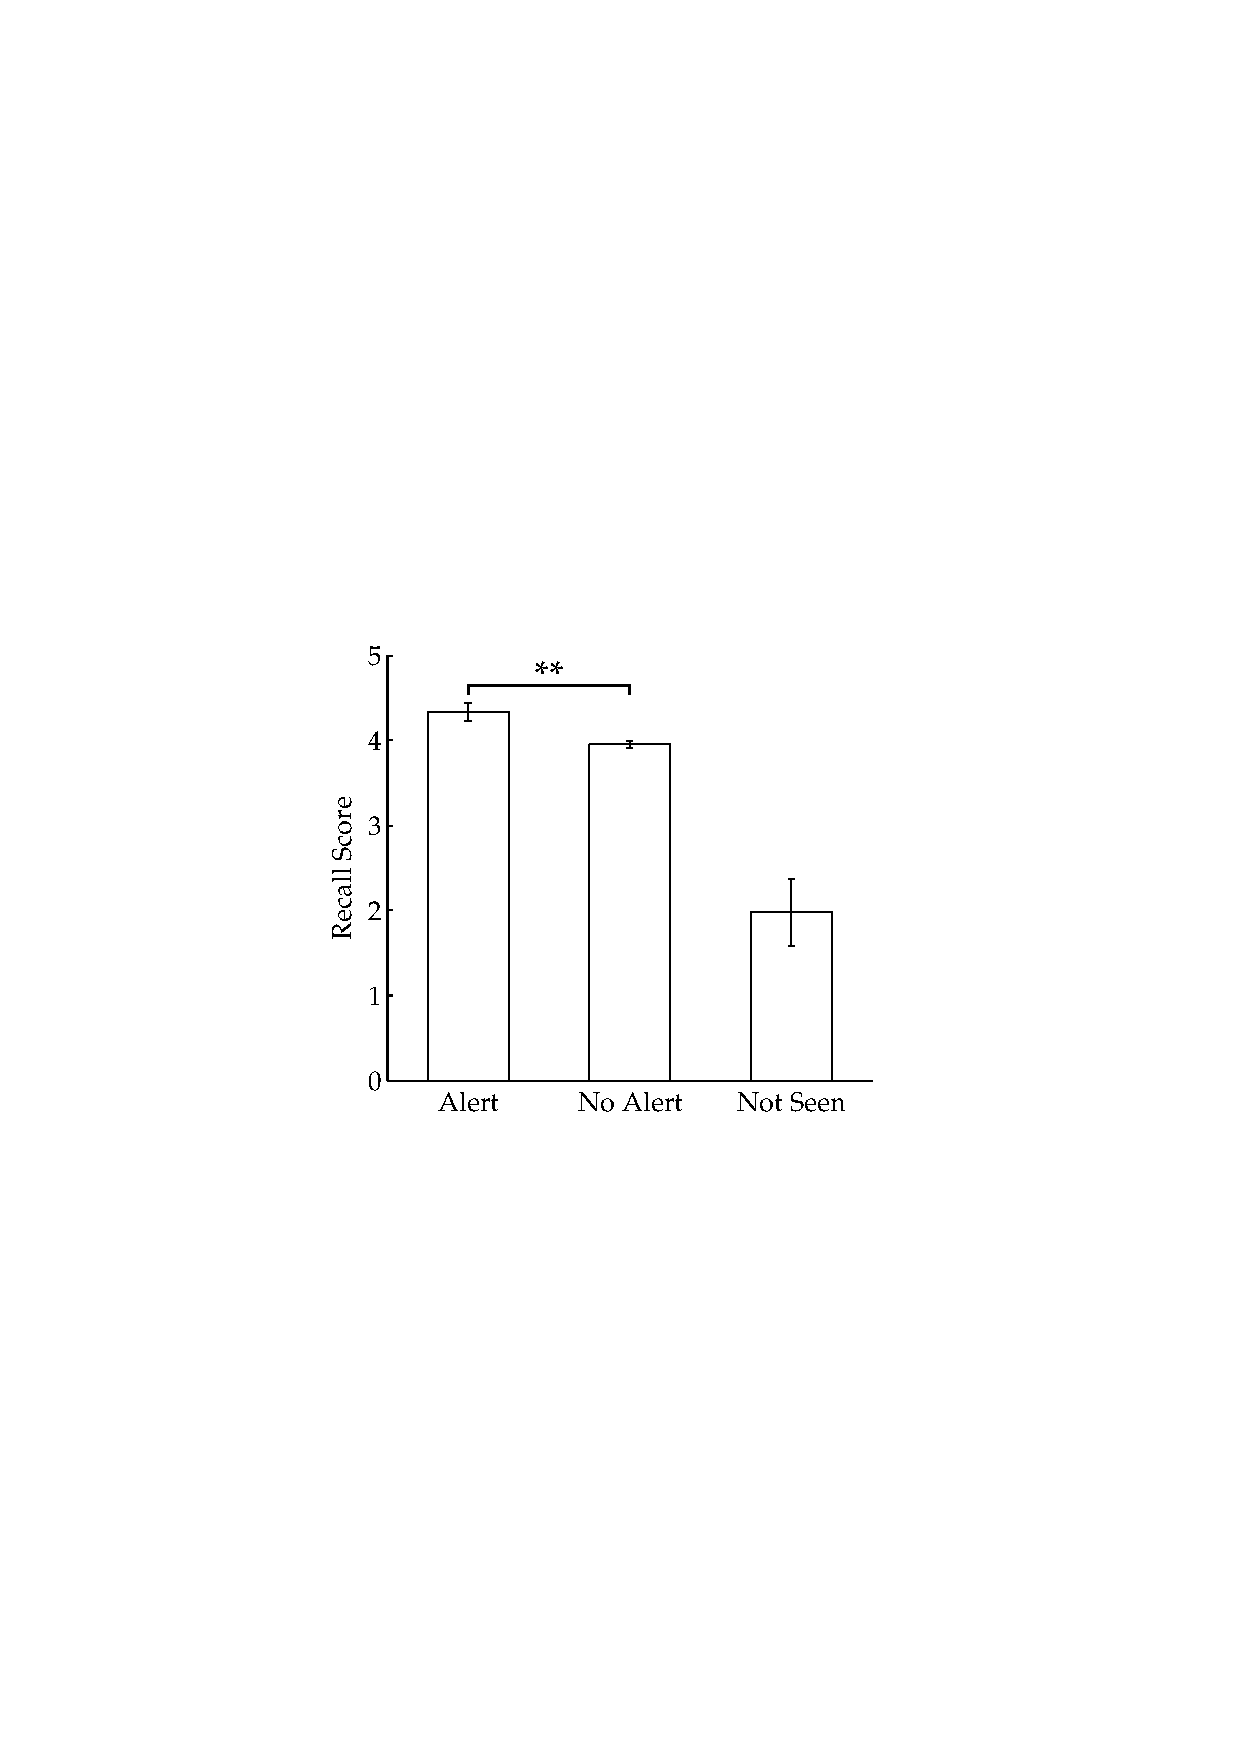
\includegraphics[width=60mm,height=54mm,trim=58mm 110mm 62mm 105mm]{./eps/memtest_alert}}
  \caption{Long-term memory test result for \textit{Alert} and \textit{No Alert} types. The arousal affects on the recall test, Alert sequences significantly get higher recall scores than No Alert sequences with the p-value of 0.0077 (p $<$ 0.01). Error bars indicate $\pm$ 2 standard errors of means (SEMs).}
  \label{fig:memtest-alert}
  \end{minipage}
\end{figure}

\begin{figure}
  \begin{minipage}{.5\textwidth}\centerline{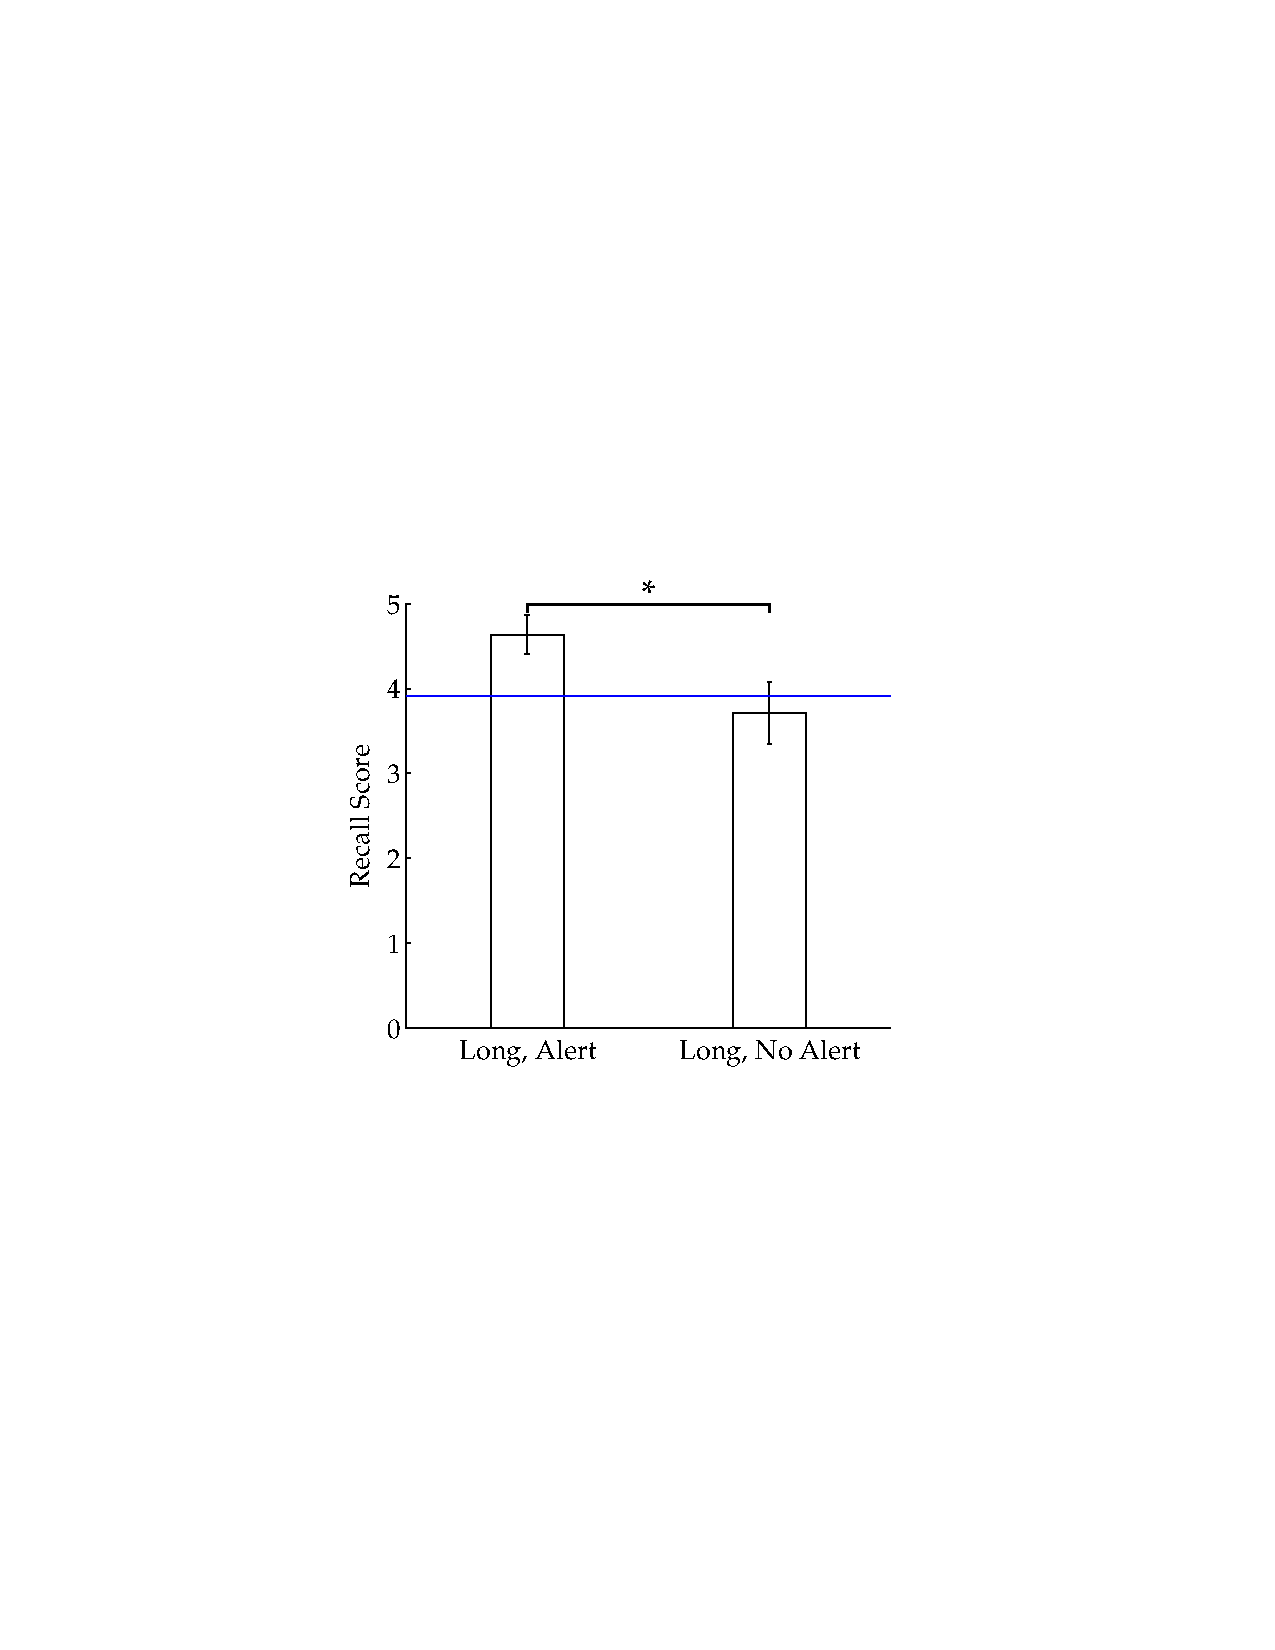
\includegraphics[width=60mm,height=54mm,trim=58mm 110mm 62mm 105mm]{./eps/memtest_long.pdf}}
  \caption{The memory test result for the long fixation which is on the \textit{Alert} sequence or the \textit{No Alert} sequence. The number of cases from 11 participants are 19 and 69, respectively. The difference between two means is statistically significant, the p-value of two-sample t-test for the \textit{Alert} type is 0.0104 ($<$ 0.05). The blue horizontal line indicates the mean scores of the long fixated sequences. Error bars indicate $\pm$ 2 SEMs.}
  \label{fig:memtest-long}
  \end{minipage}

  \vskip 0.28in

  \begin{minipage}{.5\textwidth}\centerline{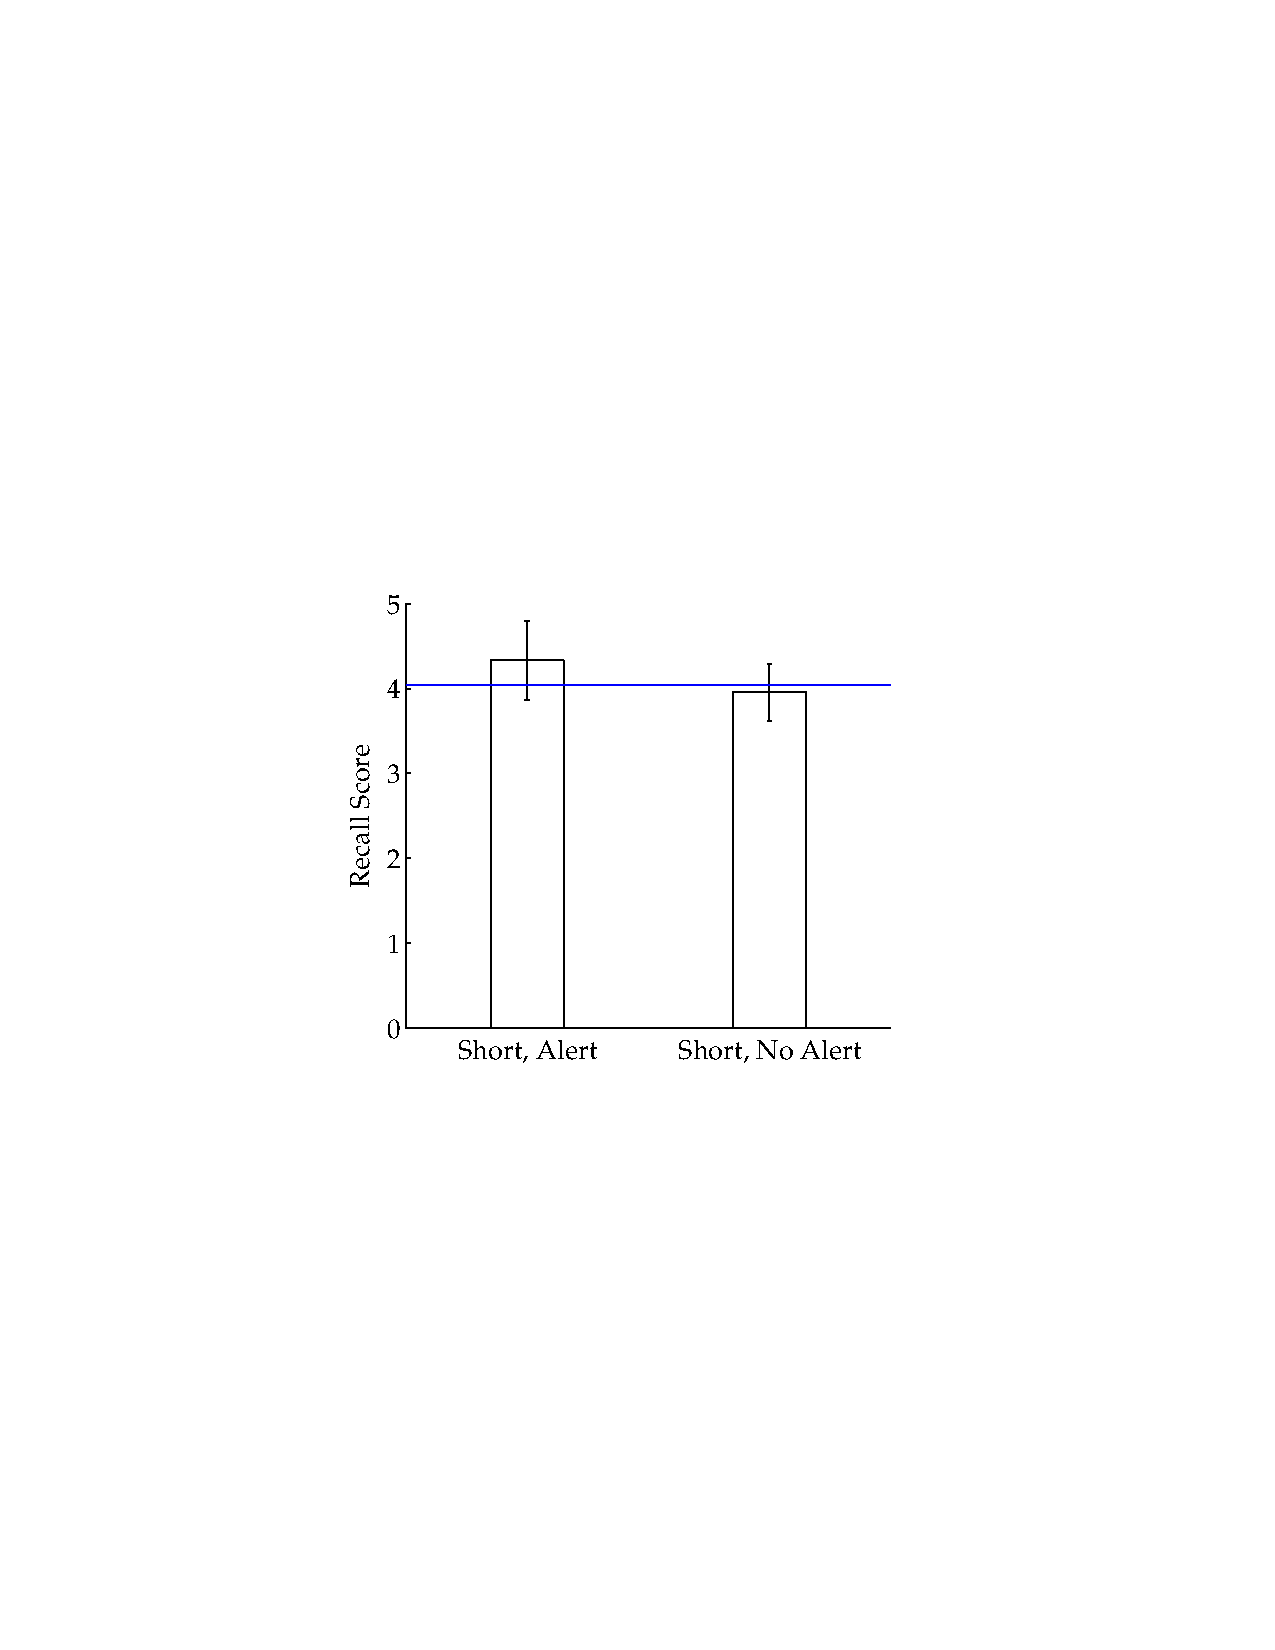
\includegraphics[width=60mm,height=54mm,trim=58mm 110mm 62mm 105mm]{./eps/memtest_short.pdf}}
  \caption{The memory test result for the short fixations which are on the \textit{Alert} sequences or the \textit{No Alert} sequences. The number of cases from 11 participants are 21 and 67, respectively. The p-value of two-sample t-test for the \textit{Alert} type is 0.2484. The blue horizontal line indicates the mean scores of the short fixated sequences. Error bars indicate $\pm$ 2 SEMs.}
  \label{fig:memtest-short}
  \end{minipage}
\end{figure}


\subsection{Gaze Variations}
\label{subsec:gaze-variations}

\begin{figure}
  \centerline{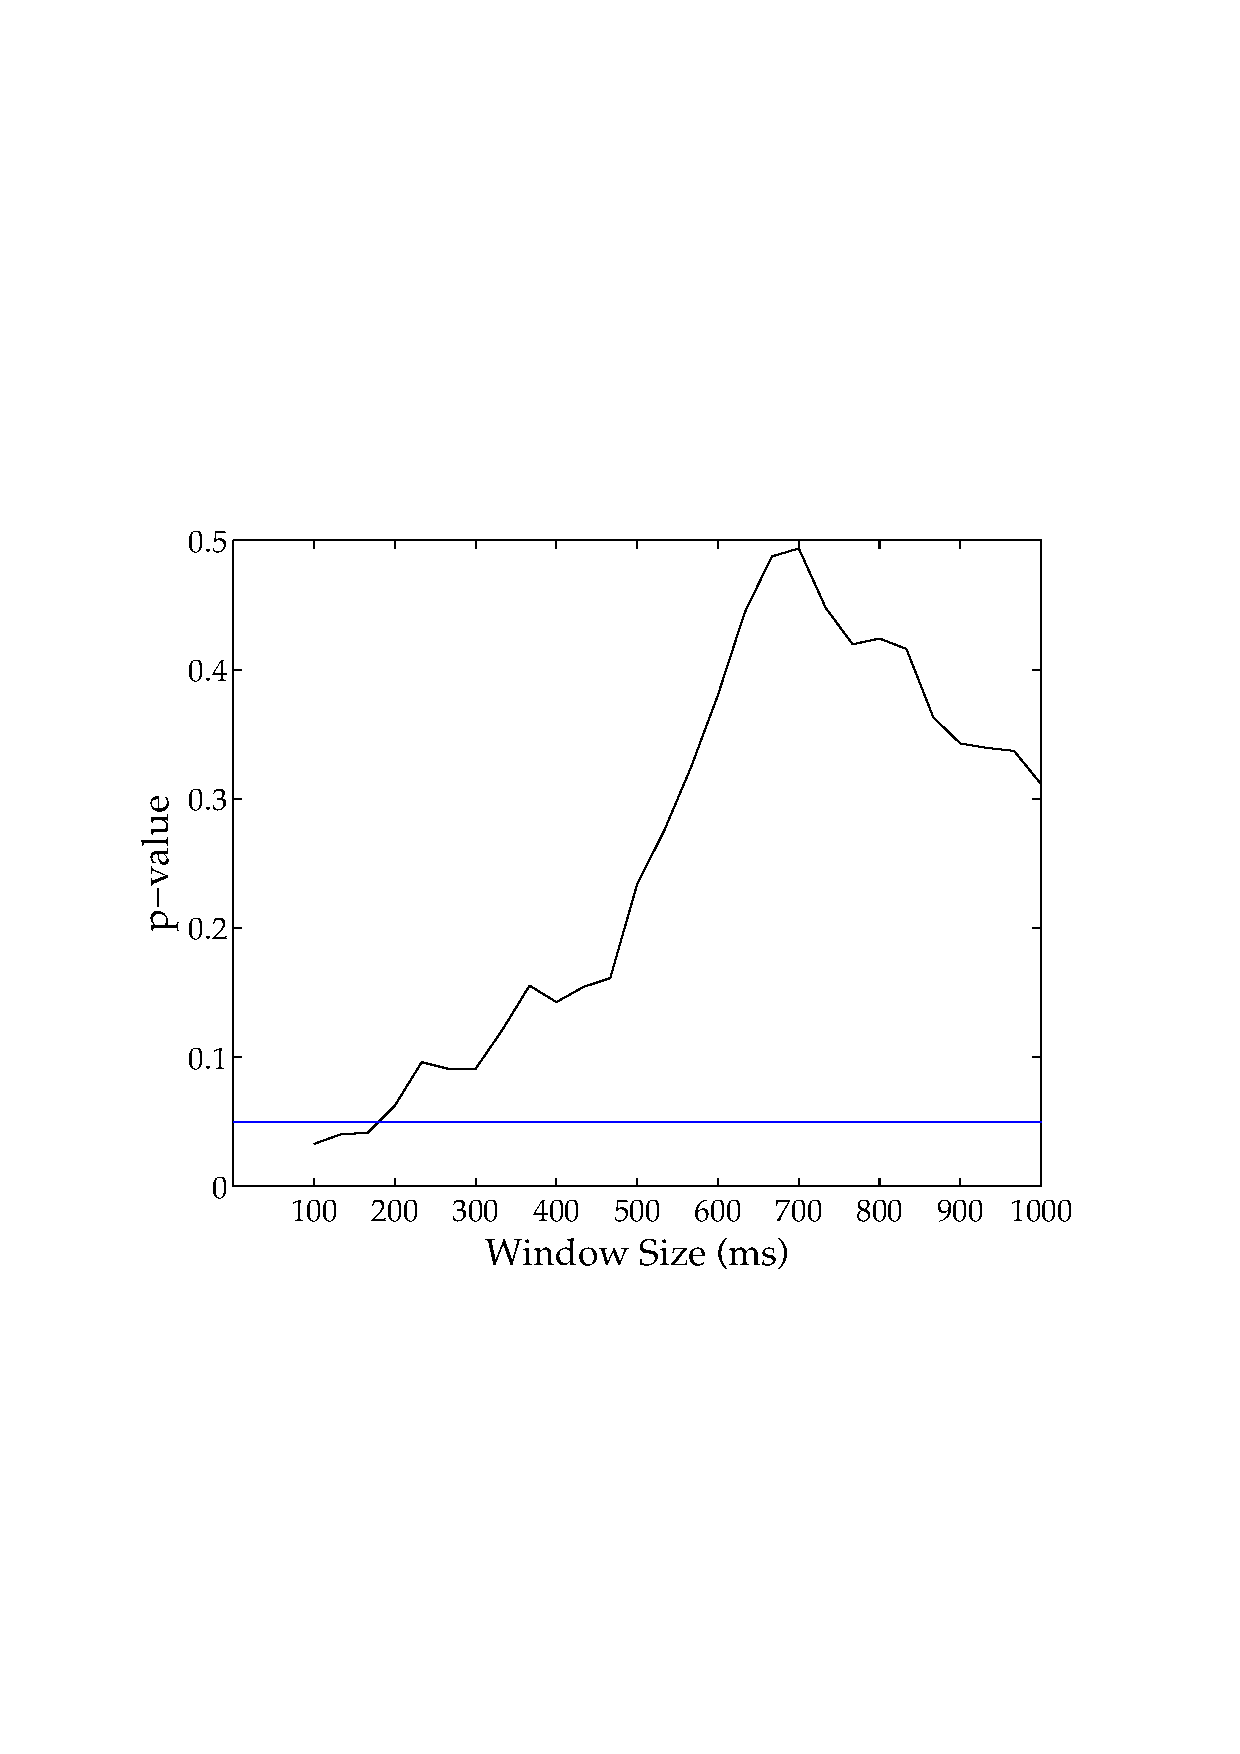
\includegraphics[width=60mm,height=65mm,trim=48mm 85mm 48mm 86mm]{./eps/gaze_var.pdf}}
  \caption{The significant levels of gaze variations with regard to the window sizes. When the window size is narrower than 200 ms, the medians of gaze variations for the \textit{Alert} sequences are significantly different from those for the \textit{No Alert} sequences (p $<$ 0.05). The blue horizontal line shows the 5\% significant level.}
  \label{fig:gaze-variation}
\end{figure}

The difference of the eye movements between the \textit{Alert} sequences and the \textit{No Alert} sequences for the long fixated is observed by the variation of gazes. Actually, the gazes keep moving in the fixation state. Because eye balls are fixed by twitching extraocular muscles. However, the most contribution to that variation is a smooth pursuit. In the smooth pursuit, the eyes are following a moving object or interesting features. Because our experimental settings do not and can not precisely define the smooth pursuit, all the eye movements slower than 30 deg/sec are candidates. 

To get the variation of the gazes excluding the variation from the smooth pursuit, we can use the window sliding technique. Varying the size of a time window, we move the time window on the time series by 1/30 second in every steps, and take the median of the variations. Figure~\ref{fig:gaze-variation} shows the significant level changes according to the change of the window size. When the window size is smaller than 200 ms, p-values are lower than 0.05. In the long fixated group, the \textit{Alert} sequences tend to have smaller gaze variations than the \textit{No Alert} sequences have, whereas the short fixated group does not show this difference.

\begin{table}[!ht]
\begin{center} 
\caption{Estimated coefficients of the linear regression model for the prediction of the recall score.} 
\vskip 0.12in
\label{tab:lr-coef} 
\begin{tabular}{lllll} 
\hline
Coef. & Estimate & SE & tStat & pValue \\ 
\hline
$\mathcal{B}_{0}$    &  4.8241   &  0.48622  &  9.9217 &  7.39e-16  \\
$\mathcal{B}_{duration}$ & -0.42214  &  0.18627  & -2.2663 &  0.025974    \\
$\mathcal{B}_{saliency}$ &  0.032642 &  0.015957 &  2.0455 &  0.043893    \\
\hline
\end{tabular} 
\end{center} 
\end{table}

\subsection{Computational Model}

Based on the study of bottom-up attention \cite{koch1985shifts}, the computational model is implemented by the saliency map-based approach \cite{itti1998model}. This model uses the visual information, i.e., intensities, color opponencies and orientations, as a source to measure the conspicuity. While reflecting some physiological evidences for the basis mechanism of visual information processing, the implement has both processing efficiency and robustness to noises. It takes an image as input, and it returns one saliency map, the matrix, note that, whose elements are normalized iteratively and nonlinearly \cite{itti2000saliency}.

Using the saliency map from the computational bottom-up attention model, we examine the association between the gaze fitness to the model and the recall score. The fitness function is described below. We use the SaliencyToolbox with default parameters for getting the saliency map to analyze, and align the gaze coordination to the area of the saliency map, which has a smaller size after sub-sampling \cite{Walther2006}.

\begin{equation}\label{eq:salsum}
X_{saliency}^{(i,j)} = \sum_{t=1}^{T} \mathcal{S}_{x_{t},y_{t}}^{(i,j,t)}
\end{equation}

In Equation~\ref{eq:salsum}, $x_{t}$ and $y_{t}$ represent the mapped gaze coordination at $t$ time in a fixation duration. $\mathcal{S}^{(i,j,t)}$ is a saliency map which is the output of the model for a given screenshot at $t$ time in the duration of a movie clip, which was given to the participant $i$ for the $j$-th sequence of the recall test.

We fit the parameters for the linear regression model for the recall scores, which is defined by Equation~\ref{eq:lm},

\begin{equation}\label{eq:lm}
Y_{score} = \mathcal{B}_{0} + \sum_{l \in \mathcal{L}} \mathcal{B}_{l} \cdot X_{l}
\end{equation}

\noindent, $\mathcal{B}$s are the coefficients of the model, and $\mathcal{L}$ is a set of features as  

\begin{equation}\label{eq:l}
\mathcal{L} = \{duration, saliency\}.
\end{equation}

$X_{duration}$ is the fixation duration in second, and $X_{saliency}$ is defined by Equation~\ref{eq:salsum}. We use only the data of the long fixations, because the short fixated sequences do not show the significant differences on the recall scores for the duration and the gaze fitness to the saliency map.

Table~\ref{tab:lr-coef} shows the estimated coefficients of the linear regression model for the prediction. All shown parameters are statistically significant, though the gaze variation is excluded for the fitting due to its unexplainable for the recall scores. The gaze fitness reasonably explains the recall score with the p-value 0.043893. The estimated value for the gaze fitness is positive, which means the recall score positively correlates with the gaze fitness in the model. Interestingly, the fixation duration, which is longer than 1400 ms, negatively correlates with the recall score, though the standard error of that is relatively high. The assessment of the model is shown in Table~\ref{tab:lr-goodness}. The number of observation is 88 for each of 11 participants rates 8 long fixated sequences, respectively. The other models, like logistic regression and non-linear regression, also examined, but they do not explain better than the linear model.



\begin{table}[!ht]
\begin{center} 
\caption{Assessment of the linear regression model.} 
\vskip 0.12in
\label{tab:lr-goodness} 
\begin{tabular}{ll} 
\hline
Attribute   & Value \\ 
\hline
\# of observations & 88 \\
Error degree of freedom & 85 \\
RMSE & 1.34 \\
$R^{2}$ & 0.106 \\
Adjusted $R^{2}$ & 0.0847 \\
F-statistics vs. constant model & 5.02 (p-value = 0.00866) \\
\hline
\end{tabular} 
\end{center} 
\end{table}

\section{Discussions}

The marginal distribution of the fixation duration shows the characteristics of the response toward the visual stimuli. The shape of the marginal distribution of fixation duration can be estimated as the exponential function though the marginal distribution of the reading fixation durations is illustrated as a left-skewed normal distribution, peaking at 180 ms. Then why reading and watching are so different from each other in this property? The first to think is the difference of the cognitive process during the fixation. Simply put, reading involves the visual processing in addition to the lexical processing. The visual process captures the letters through the retina, Lateral Geniculate Nucleus (LGN) and the primary visual cortex. Then the information of the letters is directed to the distributed lexical processing areas. Though skipping is occasionally occurred while reading, those serial processes spend some latency time. Since reading is an active task, the decision that when to move and where to move to a next word, is actively and consciously made comparing to watching task, those latencies tend to be preserved the normative shape. By the way, watching the video has a different condition. The lexical processes are typically not needed, which are heavy tasks in time. Also the video stimuli are passive in regard to the temporal aspect. Therefore the generation of the long fixation duration is sufficiently constrained by the duration of the stimulus, at the same time, the content of the stimulus. 

We recap the visual constraints which trigger the long fixation durations as three types in Table~\ref{tab:long-fixation-types}. The \textit{Alerted} is an ongoing urgent situation that makes the eyes fixates an object which is thought to be a cause or a factor. This type potentially induces the emotional arousal. The second type is the \textit{Successive}. It looks like the successive appearing of the objects keeps the fixation longer, however, the interpretation that the successive absence of the other attracting elements just lets the fixation persist is also possible. The \textit{Stationary} shows indifferent sequences and there is no significant change. Many sequences show calm and relaxed or depressed situation. Emotionally, the opposite of \textit{Alerted}. After all, what is the meaning of the long fixation durations on the video stimuli? Despite of the fact that it could be a latency time to process the cognitive information of the visual stimuli, in the other perspective, it is an waiting time to the potentially salient moment on that eye position. The waiting on the prospective location for a dramatic change or a new event is an efficient way of information processing.

Though the long fixation itself does not describe the presence of the cognitive process to memorize, in the condition of the long fixation, the arousal effect is remarkable than the others in the condition of the short fixation. As we discuss before, the long fixation is induced by active taking or passive exposure. For the cause of the long fixation is relatively well established by those two factors, the arousal effect on the long fixation is noticeable, but for the cause of the short fixation is complex and vague, the arousal effect on the short fixation is not observable.

The characteristics of the eye movement on the arousal effect are probed by the statistical method and the computational attention model. First of all, we hypothesize on that the variation of gaze points indicates the observable response of the arousal effect in the condition of the long fixation. As we report in Subsection~\nameref{subsec:gaze-variations}, the gaze variation on the alerted sequences are smaller than those on the other case, when the window size is shorter than 200 ms, to minimize the variation from the slow pursuit. Yet, the gaze variation does not have a statistical power to predict on the recall score, which is the measurement for the long-term memory. Though the arousal stimuli associate with the long-term memory \cite{Cahill1996amyg,Cahill1998baso}, we conclude that the gaze variation explains only the arousal effect, not until the further cognitive process. 

Second, we establish the linear model to predict the recall score using the computational attention model by \citeA{itti1998model} in addition to the fixation duration. Also, for the short fixated sequences, we cannot find the variables, so we assert to use the observed data of the long fixated sequences. Although we formulate the simple summation of saliency scores for the prediction, it shows the significant level of prediction. And, when the fixation duration is longer than 1400 ms, the longer fixate, the less memorize. Though for the standard error is bit high, we have to be cautious enough to it. 

The value of the adjusted $R^{2}$ for the model reminds us that the information of eye movement should carefully use to estimate the cognitive process. As well as, there is the limitation of the analysis coverage, for the majority of the eye movement is the short fixated ones. 

However, the investigation is not complete. We look forward to have more distinct features. A temporal modeling using the salient detectors \cite{marr1980,canny1986} and the optic flow \cite{koenderink1986} may be a promising option. Moreover, the cognitive modeling for the scene comprehension, which is related to the emotion-based reaction guides us into the diffent level of a methodological stage. As we discussed, the long fixations are constrained by the visual content of the video stimuli, and with regard to that, the response of the gaze direction selects what it acquires in a reciprocal manner \cite{zhang2013}. Additionally, the estimation of the eye movement is viable on top of this reciprocally anticipatory model \cite{robert1985anticipatory}. The serial information of the fixation positions enables us to intelligently select the portion of the visual features on the scene, like a human, it can be a breakthrough for the cognitive modeling on the endless stream of the visual information.


\section{Conclusions}

We study the characteristics of the eye movements through the marginal distribution of fixation durations. We notice that the marginal distribution of fixation durations for the video stimuli has a form which is different from the marginal distribution of fixation durations for the reading materials. The behavioral basis for the difference may attribute to the lighter load for the cognitive process and the temporal and spatial constraints which are given by the video stimuli. Those constraints are summed up as three distinctive types, Alerted, Successive and Stationary. We find the arousal effect only for the long fixated sequences. The small gaze variation for the long fixation indicates an active response to the arousal stimuli. However, the gaze variation does not help to estimate for the recall score, among the long fixations, just the fixation duration and the saliency-probing activity are significant to model. The computational model partly describes the embodied cognitive framework with the perception-action cycling.


\section{Acknowledgments}

This work was supported by the National Research Foundation of Korea (NRF) grant funded by the Korea government (MSIP) (NRF-2010-0017734-Videome),
supported in part by ICT R\&D program funded by the Korea government (MSIP/IITP) (10035348-mLife, 14-824-09-014, 10044009-HRI.MESSI).

\bibliographystyle{apacite}

\setlength{\bibleftmargin}{.125in}
\setlength{\bibindent}{-\bibleftmargin}

\bibliography{kim2015activelong}

\end{document}
